\clearpage
\section{Arduino Quantum Receiver}

\begin{refsection}

\begin{tcolorbox}	
\begin{tabular}{p{2.75cm} p{0.2cm} p{10.5cm}} 	
\textbf{Student Name}  &:&  Eduardo Fernandes (2019/06/15 - 2019/09/14)\\
\textbf{Goal}          &:& Implement the QKD reception module in an Arduino (Coincidence Detector, QBER, Source and Sink blocks).\\
\textbf{Directory}              &:& sdf/arduino\_quantum\_rx
\end{tabular}
\end{tcolorbox}


\subsection{Simulation Analysis - QKD reception module}

\begin{figure}[H]
	\centering
	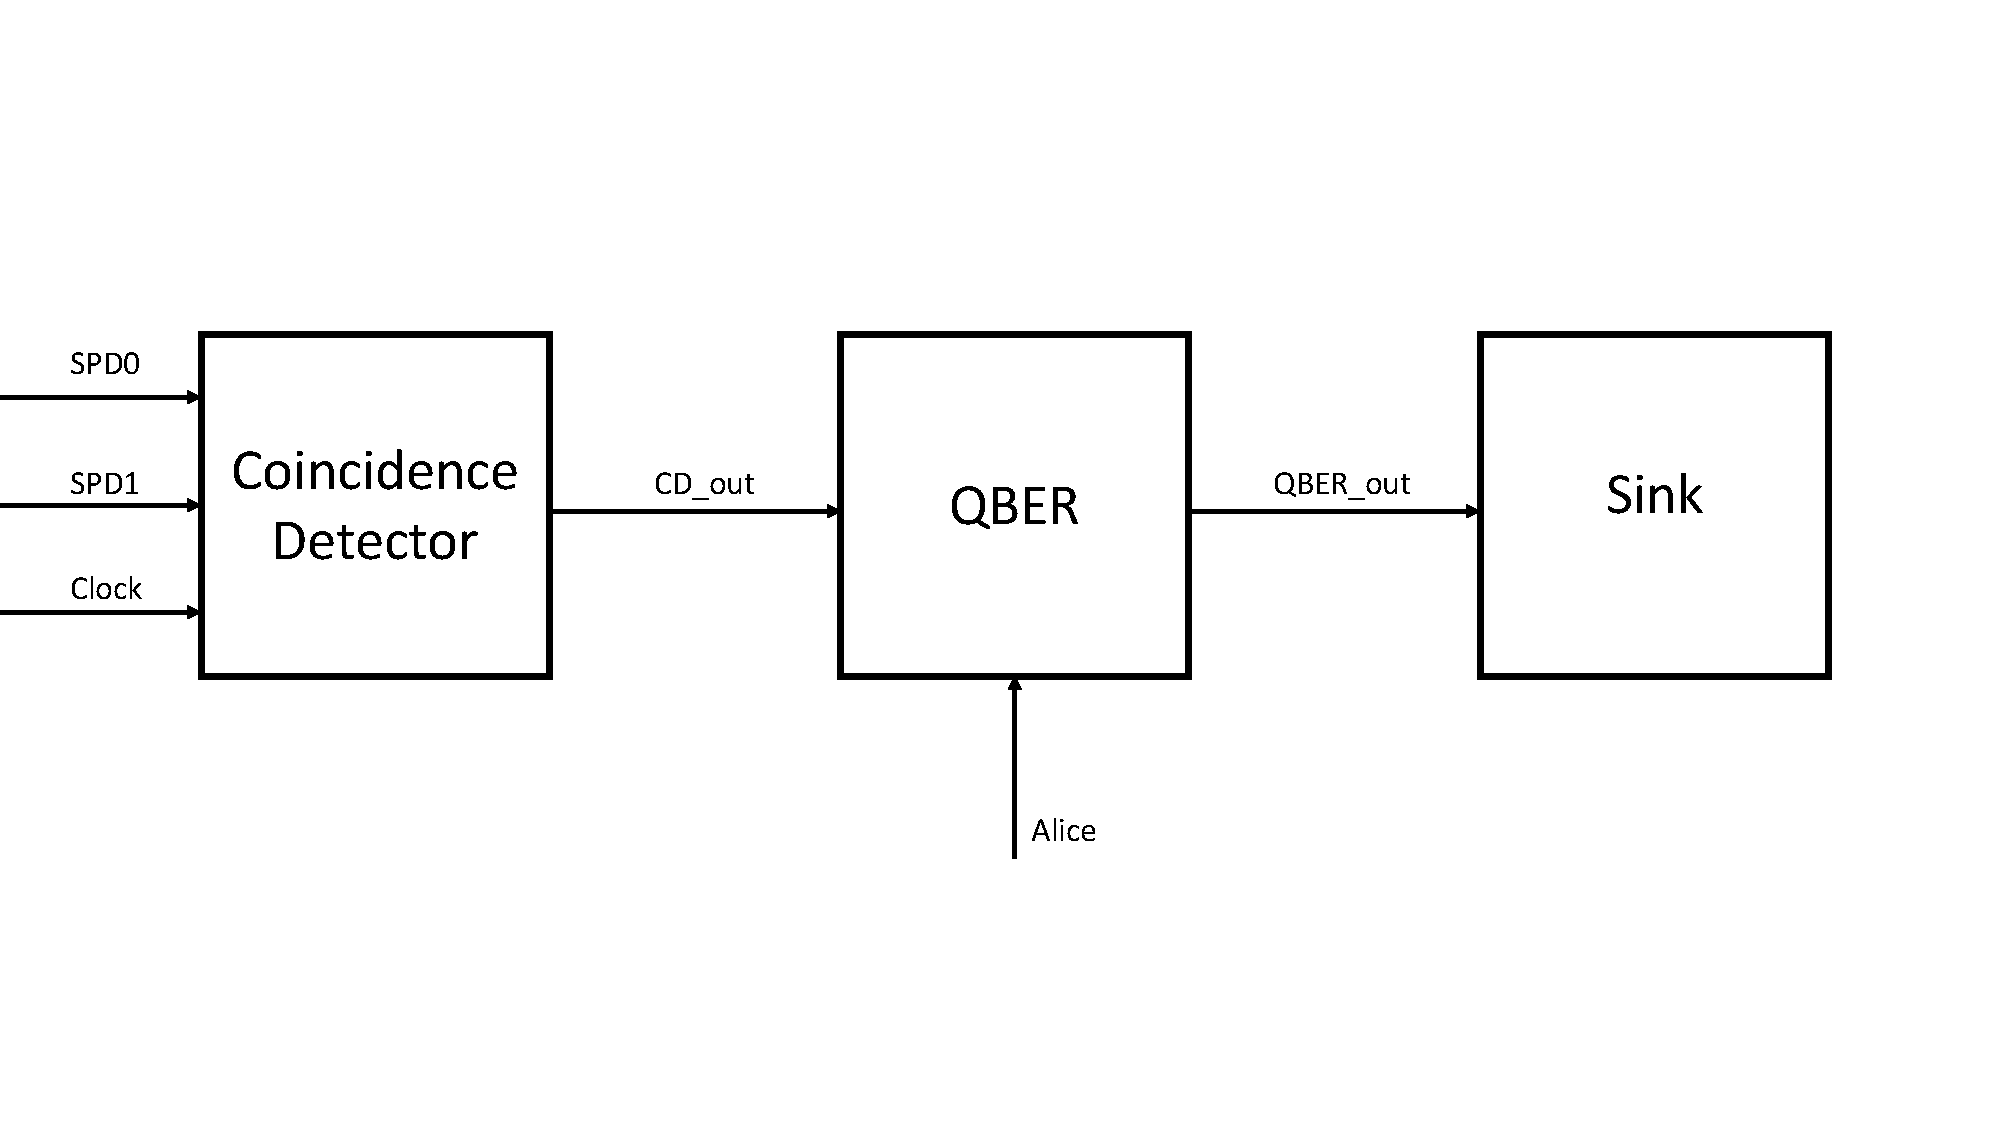
\includegraphics[width=1\linewidth]{./sdf/arduino_quantum_rx/figures/generalDiagram.pdf}
	\caption{General block diagram of QKD a quantum receiver module.}
	\label{fig:arduino}
\end{figure}

This system emulates the QKD reception module of a quantum communication system. It is comprised by three main blocks. The first is the coincidence detector  which contains three inputs: the signals provenient from the single-photon detectors 0 and 1 and a clock signal used to keep all blocks synchronized, as it provides the sampling frequency. In addition, this block outputs a signal containing a state corresponding to the input values. That signal will be the input of the next block, the QBER, this block compares two input binary signals, one provenient from the coincidence detector and one other coming directly from Alice's side, and outputs a binary signal with a zero if both input bits are equal and a one if they differ. Additionally, this block does statistical analysis on the QBER and outputs a file with the results of this analysis. Finally, the output signal of the QBER block enters a Sink block, not generating any output. 

\subsection{Emulation in NetXPTO Simulator}

\vspace{11pt}

\begin{figure}[H]
	\centering
	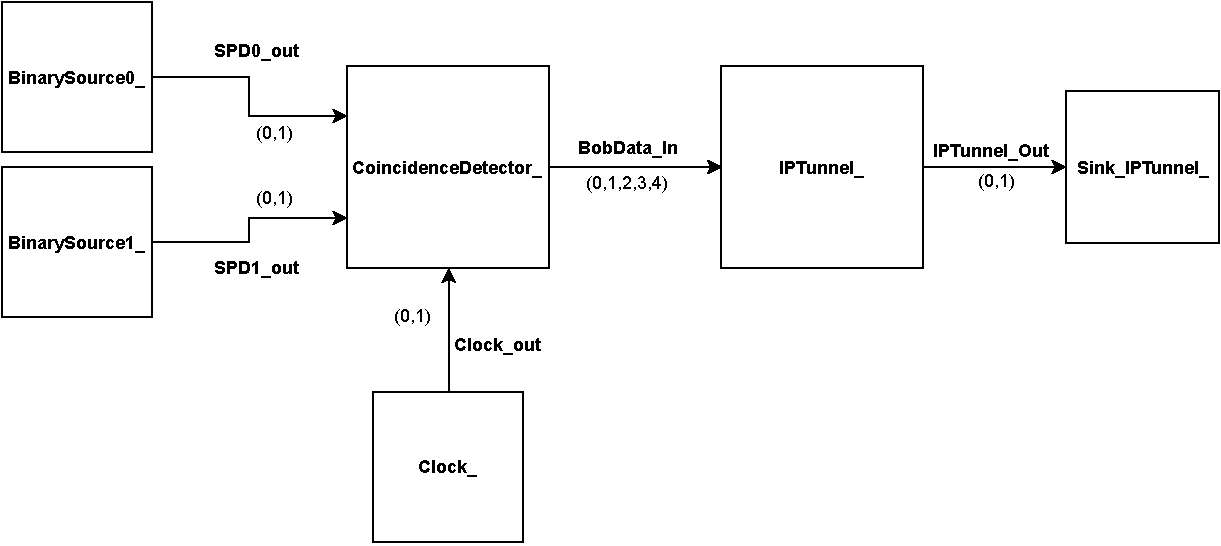
\includegraphics[width=0.9\linewidth]{./sdf/arduino_quantum_rx/figures/NetXPTO_implementation.pdf}
	\caption{Block diagram of a quantum receiver system emulated in NetXPTO.}
	\label{fig:netxpto}
\end{figure}

Here are presented and described the implementation of 6 modules needed. The first two are the BinarySource0\_ and the BinarySource1\_ which emulate the received signals provenient from the single-photon detectors 0 and 1, respectively. These signals are the inputs of the CoincidenceDetector\_ block, which in its turn, outputs a real signal that has five possible values: 5 if it is a control qubit (which should be discarded by the upper layer), 3 if no-click has been detected, 2 if both detectors clicked, 1 if bit one was measured, and finally, 0 if bit zero was measured. Next, we have the BinarySource2\_ block which has a binary output signal representing the measured value that arrives from the quantum channel from Alice side. Another existent block is the QBER\_ which is responsible for some of the post processing tasks, more specifically, the QBER estimation and outputs a real signal with the quantum channel QBER. Finally there is the Sink\_QBER\_ blocks, which, accpets one binary input signal provenient from the QBER\_ block and does not produce any output signals, it simply takes samples out of the circular buffer until it is empty.\\ \\

The following input parameters were defined for the blocks listed in figure \ref{fig:netxpto}:

\begin{itemize}
	\item BinarySource0\_:
	\begin{itemize}
		\item setMode(BinarySourceMode::DeterministicCyclic)
		\item setBitPeriod(1e-11)
		\item setBitStream("1")
		\item setNumberOfBits(10000);
	\end{itemize}
	\clearpage
	\item BinarySource1\_:
	\begin{itemize}
		\item setMode(BinarySourceMode::DeterministicCyclic)
		\item setBitPeriod(1e-11)
		\item setBitStream("0")
		\item setNumberOfBits(10000);
	\end{itemize}
	
	\item BinarySource2\_:
	\begin{itemize}
		\item setMode(BinarySourceMode::DeterministicCyclic)
		\item setBitPeriod(1e-11)
		\item setBitStream("1")
		\item setNumberOfBits(10000);
	\end{itemize}
	
	\item CoincidenceDetector\_;
	
	\item QBER\_;
	
	\item QBER\_Sink\_.
\end{itemize}





\subsection{Simulation Analysis - Arduino Implementation}

In order to utilize the same project running over NetXPTO simulator using Arduino some changes in the source code had to be made once this technology uses C and C++ languages while relying on special rules of code structuring.

The outputs to the console have to be made through the arduino serial monitor using the function Serial.print() instead of making use of the class cout; 

\subsection{Open Issues}

% bibliographic references for the section ----------------------------
\clearpage
\printbibliography[heading=subbibliography]
\end{refsection}
\addcontentsline{toc}{subsection}{Bibliography}
\cleardoublepage
% ---------------------------------------------------------------------
